\chapter{Проблема формалізації голосової інформації в системах диспетчерського контролю за рухом автотранспорту} \label{chapt1}

%\section{Інформаційні технології в системах дистрибуції} \label{sect1_1}

\section{Сучасний етап автоматизації голосового управління в організаційно-технічних системах} \label{sect1_2}

Голосове управління уже має певну історію використання в транспортній сфері. Передові автоконцерни світу, такі як Ford Motor Company, BMW AG, Daimler AG прагнуть підвищити безпеку та комфорт водія, тому створюють можливість керування бортовою електронікою за допомогою голосу \cite{Kravchenko_2009}. Перша подібна система, що мала назву Linguatronic, була представлена інженерами Mercedes в автомобілі S-класу в 1996 році \cite{Heisterkamp_2001}. Вона реалізувала голосове управління функціями вбудованого телефону та адресної книги, радіо та CD-програвача, а також кондиціонеру. Fiat, працюючи з Microsoft, розробив систему з ініціацією водієм Blue\&Me, в якій перед початком мовної команди треба було натиснути кнопку на кермі. Інженери BMW також розробили систему з ініціацією водієм, що була інтегрована з їх системою управління бортовою електронікою iDrive. Honda, використовуючи систему розпізнавання мови IBM ViaVoice, надала можливість керування GPS навігацією для голосового вказання адреси прибуття \cite{Jonsson_2009}.

Крім того, за наявності достатньо потужної системи, голосову взаємодію з водієм можна використовувати для підтримання діалогу під час руху вночі, аби не дати водію заснути \cite{Kravchenko_2012}.

Також проводилися дослідження з розробки систем мовного управління бортовим обладнанням літаків, але через високі вимоги до швидкості та якості розпізнавання, особливо за наявності потужних шумів та перешкод, вони ще досі не були запроваджені \cite{Korsun_2013}.

Використання таких часткових функцій голосового управління, які підвищують комфорт водія, також повинно мати певний позитивний ефект. Проте ці функції не забезпечують оптимізації саме процесів диспетчерського контролю за рухом автотранспорту.

\section{Автоматизація управління в системах диспетчерського контролю за виконанням доставок автотранспортом} \label{sect1_3}

Дистрибуція — це діяльність, повʼязана з отриманням продукції, її зберіганням до моменту отримання замовлення і наступної доставки до клієнтів. Управління дистрибуцією включає в себе планування, організацію та контроль. Проблема управління ланцюгом поставок є надзвичайно актуальною в дистрибуції та логістиці \cite{Speranza_2018}, особливо питання стійкості \cite{Koberg_2018,Jia_2018,Bastas_2019,Wen_2018,Sullet_2018} та екологічності \cite{Tseng_2019,Papetti_2019,Hoehne_2017}. Особливо важливим є етап «останньої милі» \cite{Baldi_2018,Gdowska_2018,Boysen_2018,Hoehne_2017,Pronello_2017,Cook_2017} та вплив інтернет магазинів на ці процеси \cite{Allen_2018,Cardenas_2017}.

Для покращення процесів доставки використовується велика кількість різноманітних інформаційних технологій, таких як RFID \cite{Prasanna_2012}, GPS \cite{Stopher_2018,Prasanna_2012} та GSM \cite{Prasanna_2012} трекери, принципи «інтернету речей» \cite{Liu_2018} та «big data» \cite{Govindan_2018}, використання додатків на смартфонах \cite{Stopher_2018}, web-системи управління ланцюгом поставок \cite{Papetti_2019} та інші.

Інформаційні технології в управлінні дистрибуцією вже достатньо розроблені для забезпечення етапів отримання продукції та її збереження, отже зараз найбільш інтенсивно йде розвиток етапу доставки продукції до кінцевих клієнтів. Зокрема розробляються системи автоматизації побудови планових маршрутів руху автотранспорту \cite{art1}, системи керування транспортним парком (TMS) та моніторинг доставок у реальному часі.

У сучасних системах автоматизації дистрибуції, доставки і керування транспортним парком достатньо розробленим є і процес автоматизації побудови планових маршрутів руху автотранспорту \cite{art1}. Він включає в себе складові врахування топології, часових параметрів точки доставки (часові вікна доступності та час, необхідний на обслуговування точки), завантаженість автомобіля, кількість доступного транспорту тощо. Проте проблема своєчасного коригування маршруту у випадках, коли реальний стан справ перестає відповідати запланованому маршруту, викликає достатньо великі витрати часу на комунікацію. Якби ці функції реалізувалися за допомогою автоматизованої голосової взаємодії, це дало б максимальний ефект для покращення управління дистрибуцією.

Велику роль в управлінні дистрибуцією відіграють процеси голосової взаємодії, які зараз активно автоматизуються для підвищення ефективності, збереження ресурсів тощо. Голосова взаємодія поділяється на безпосередню та із залученням інформаційних технологій. Інформаційні технології в цьому контексті можуть слугувати лише засобом забезпечення звʼязку, що саме по собі може давати ефект, але найкращий результат можна отримати, якщо внести певні автоматизації голосової взаємодії.

Для управління доставкою вантажів у дистрибуції вкрай важливим є етап моніторингу руху автомобілів у режимі реального часу. Це дозволяє аналізувати ефективність водія, а також передбачати певні небажані інциденти. Для такого моніторингу використовують GPS дані руху автомобіля\cite{Gonzalez_2013,Comendador_2012}. На жаль лише GPS треку не достатньо для однозначного розуміння стану справ. З треку тільки й видно, що водій був біля точки доставки, але не зрозуміло, чи виконана доставка, чи з якихось причин відмінена. З треку ясно, що за поточної швидкості водій відстає від плану та не встигає на наступну точку, але не зрозумілі причини відставання та чи має водій можливість надолужити втрачений час. Для отримання цієї інформації необхідна додаткова комунікація водія з диспетчером. Але дзвінок по телефону чи, ще гірше, комунікація через якийсь візуальний інтерфейс у смартфоні забирає певний час та знижує концентрацію уваги водія на дорозі, що може спричинити ДТП. Тому потрібна система, яка б дала змогу виявляти необхідну інформацію в голосових даних водія і відправляти її диспетчеру у формалізованому вигляді.

Найбільш подібна до цього система Pick-by-Voice \cite{Pick-to-Voice}. Це система, що використовується в іншій сфері управління дистрибуцією — управлінні складськими процесами. Pick-by-Voice дає змогу відбірнику по черзі отримувати голосові команди у вигляді: де, що і в якій кількості треба відібрати, а також у формі діалогу повідомляти про необхідність повторити завдання чи переходити до наступного тощо. Така система дає змогу звільнити руки та очі відбірнику і в цілому збільшити його ефективність на 35\% \cite{Baumann_2012}.

На жаль для управління транспортними доставками потрібна більш складна система, ніж наявні можливості Pick-by-Voice, адже вона повинна мати суттєво більший спектр необхідних для розпізнавання команд. У передових системах управління міськими доставками вантажів (urban freight distribution) важливим параметром є часові вікна доставки \cite{Quak_2006}. Такий параметр зразу вводить цілу низку додаткової інформації, яку треба передати від водія до диспетчера — наскільки вчасно були виконані доставки, скільки часу було витрачено на кожну з них, відставання від плану внаслідок пробок або інших непередбачуваних обставин тощо. Більше того, система повинна забезпечувати взаємодію з диспетчером у режимі реального часу, а не відтворювати заданий заздалегідь перелік завдань.

Таким чином, очевидною стає необхідність упровадження системи голосової взаємодії між водієм та диспетчером для отримання необхідної інформації від водія в мовній формі та автоматизації управління дистрибуцією.

\section{Сучасні досягнення формалізації голосової інформації} \label{sect1_4}

\subsection{Попередня обробка голосової інформації та виділення ознак}

\subsubsection{Перетворення Фурʼє}

Перетворення Фурʼє використовується в багатьох областях науки, в тому числі і в мовних технологіях. В області обробки мовних сигналів перетворення Фурʼє розглядається як перетворення сигналу з часової в частотну область і розкладання його на частотні складові. У завданнях цифрової обробки часто використовують дискретне перетворення Фурʼє, так як мовний сигнал часто представляють в дискретному вигляді, як суму гармонічних складових.

Побудова спектра з використанням дискретного перетворення Фурʼє дозволяє компактно і наочно представити інформацію про мовний сигнал. Однак в спектральному вигляді неможливо детально аналізувати короткочасні локальні особливості, що є серйозним недоліком дискретного перетворення Фурʼє \cite{Сергиенко_2002}.

\subsubsection{Вейвлет-перетворення}

Незважаючи на широку практичну популярність перетворення Фурʼє, останнім часом багато завдань в області обробки мовних сигналів реалізуються з використанням вейвлет-перетворення. Вейвлетом (материнським вейвлетом) називається деяка функція, добре локалізована (тобто зосереджена в невеликій околиці деякої точки і різко спадна до нуля в міру віддалення від неї) як в часовій, так і в частотній області. До материнського вейвлету застосовуються дві операції: зсування (переміщення області локалізації в часі) і масштабування (розтягування або стиснення, тобто переміщення області його локалізації за частотою).

Сутність вейвлет-перетворення полягає в розбитті сигналу на масштабовані і зсунуті по осі часу версії материнського вейвлета та у обчисленні коефіцієнтів кореляції ділянок вихідного сигналу і версій вейвлета на заданому масштабі. В результаті виходить набір коефіцієнтів, що показують, наскільки поведінка сигналу в даний момент часу схоже на поведінку вейвлета на даному масштабі, тобто вейвлет-коефіцієнти відображають близькість сигналу до вейвлету даного масштабу. Чим ближче вигляд аналізованого сигналу в околиці даного моменту часу до вигляду вейвлета, тим більше абсолютне значення має відповідний коефіцієнт.

Використання зсуву і масштабування в частотно-часової області дозволяє аналізувати мовні сигнали на різних масштабах і точно визначати положення їхніх характерних особливостей в часі. Найбільш часто зустрічаються вейвлет-функції в задачах обробки мовних сигналів: вейвлет Хаара, вейвлет Добеши, вейвлет «Мексиканский капелюх», вейвлет Марлет (комплексний базис) \cite{Майдан_2007}.

Вейвлет-перетворення має істотні переваги в порівнянні з перетворенням Фурʼє. Це випливає з можливості аналізувати короткочасні локальні особливості сигналів, наприклад, короткі сплески чи провали, розриви та сходинки і тому подібне.

\subsubsection{Перетворення Гільберта-Хуанга}

Відомо, що для адаптивного аналізу мовних сигналів за допомогою вейвлет-перетворення необхідно використовувати апріорну інформацію - функцію материнського вейвлета. Питання про вибір відповідної функції вейвлета на основі характеристик аналізованого сигналу не завжди є однозначним. Для вирішення проблеми адаптивності використовується новий метод обробки, заснований на перетворенні Гільберта-Хуанга. Основною перевагою даного методу є висока адаптивність, що виявляється в тому, що базисні функції, які використовуються при розкладанні звуку, витягуються безпосередньо з самого вихідного сигналу і дозволяють враховувати тільки йому властиві особливості.

Перетворення Гільберта-Хуанга включає два основних етапи: розкладання сигналу на компоненти --- декомпозиція на емпіричні моди \cite{Huang_1998,Tychkov_2013} та формування за отриманими емпіричними модами спектру Гільберта \cite{Huang_2013}.

В результаті перетворення Гільберта-Хуанга мовний сигнал представляється в частотно-енергетично-часової області, що дозволяє виявити приховані модуляції і області концентрації енергії, які дозволяють аналізувати як глобальні, так і локальні властивості сигналів і вимагають менших обчислювальних витрат.

\subsubsection{Кепстральний аналіз}

В області обробки мовних сигналів кепстральний аналіз отримав широку популярність, яку можна пояснити перевагою стиснення інформації про мовний сигнал при переході в частотну область обробки.

Відомо, що при перетворенні сигналу з часової області в частотну інформація виявляється більш докладною, наочною та компактною. Виходячи із зазначених переваг спектрального представлення інформації і народилася ідея кепстрального аналізу: заміна в спектрі вісі частоти на вісь часу, іншими словами, уявити, що спектр є просто сигналом. Таким чином, зʼявиться можливість уявити вихідну спектральную інформацію ще більш компактно, коли кожен гармонійний ряд вихідного спектра буде представлений всього однією складовою в кепстра.

На сьогоднішній день загальноприйнято вважати, що кепстр - це спектр логарифма спектра вихідного сигналу, тобто початковий спектр повинен бути представлений в логарифмічному масштабі \cite{Козлов_2013}.

Кепстральний аналіз в задачах обробки мовних сигналів заснований на виділенні кепстральних коефіцієнтів на мел-шкалі, названих мел-частотними кепстральними коефіцієнтами. Метод отримання мел-частотних кепстральних коефіцієнтів заснований на моделі функціонування органів слуху людини і використовує частотну шкалу в мелах, яка моделює частотну чутливість людського вуха \cite{Huang_2001}.

\subsubsection{Лінійне передбачення}

Лінійне передбачення є одним з найбільш використовуваних методів в задачах обробки мовних сигналів. Модель лінійного передбачення ґрунтується на припущенні, що будь-який відлік мовного сигналу $s(n)$ можна приблизно оцінити лінійної комбінацією деякого числа $p$ попередніх йому відліків \cite{Любимов_1995}.

Існують два основні методи визначення лінійного передбачення, які називаються автокорреляційним і ковариаційним методами рішення відповідно. Обидва методи використовують представлення сигналу у часовій області. Коефіцієнти передбачення визначають частотну характеристику фільтра, що характеризує стан голосового тракту в певний момент часу. З одного боку, даний момент не може бути точно локалізований, з іншого боку, точність сильно залежить від стаціонарності досліджуваного сигналу. Іншими словами, дані методи обчислення забезпечують отримання деякої середньої оцінки аналізованої ділянки сигналу в частотно-часової області.

\subsubsection{Кореляційний аналіз}

Кореляційний аналіз --- це визначення взаємозвʼязку двох або декількох статичних величин (або величин, які можна з деяким допустимим ступенем точності вважати такими). Математичною мірою кореляції двох величин служить коефіцієнт кореляції. Кореляційний аналіз статистичних даних досить популярний в обробці мовних сигналів. Популярність методу обумовлена ​​двома моментами: коефіцієнти кореляції відносно прості в підрахунку і їх застосування не вимагає спеціальної математичної підготовки. Що стосується завдань обробки мовних сигналів, ключовими поняттями кореляційного аналізу стають автокореляційні та взаємокореляційні функції \cite{Баскаков_2001}.

Автокореляційна функція визначає статистичний взаємозвʼязок між величинами з одного мовного сигналу, розкладеного в ряд, але взятих із зсувом. Взаємокорреляційна функція визначає ступінь кореляції двох послідовностей значень мовних сигналів, розкладених в ряди, також взятих із зсувом.

\subsection{Перетворення голосової інформації в текстову}

\subsubsection{Нейронні мережі}

Одним з найбільш ефективних методів розпізнавання мовних сигналів є метод з використанням нейронних мереж, що структурно складаються з нейронів та організованими між ними звʼязків. Нейрон являє собою елемент нейронної мережі. За аналогією з нервовими клітинами головного мозку він може бути в двох станах: збудження або гальмування. Нейрони мають різні звʼязки між собою: синапси --- односпрямовані вхідні звʼязки, аксони --- вихідні звʼязки нейрона, за якими сигнали (збудження або гальмування) надходять на синапси наступних нейронів.

Кожна однонаправлена звʼязок характеризується вагою $w_i$ (величиною синаптичного звʼязку), який за фізичному змісту еквівалентні до електричної провідності. Додатні та відʼємні значення $w_i$ відповідають збудженому або загальмованому стану синапсів. Сума всіх входів визначає поточний стан нейрона \cite{Чураков_2014}.

При використанні нейронних мереж в задачі розпізнавання мовних сигналах необхідно побудувати відповідну певну для цього завдання мережу, далі навчити її множині мовних сигналів --- підібрати вагові коефіцієнти синапсів для досягнення мінімізації кількості помилок.

\subsubsection{Приховані Марковські моделі}

Одним з найбільш ефективних методів обробки (розпізнавання) мовних сигналів є метод з використанням прихованих Марковських моделей. Приховані Марковські моделі --- статистична модель, що імітує роботу процесу, схожого на Марковський процес з невідомими параметрами. Головним завданням прихованих Марковських моделей є визначення (розгадування) невідомих параметрів на основі спостережуваних. Отримані параметри можуть бути використані в подальшому аналізі, наприклад, для розпізнавання образів.

Застосування прихованих Марковських моделей в розпізнаванні ґрунтується на наступних припущеннях \cite{Огнев_2013}:

\begin{itemize}
	\item мовний сигнал може бути сегментований на фрагменти (стани), всередині яких сигнал може розглядатися як стаціонарний. Перехід між цими станами здійснюється миттєво;
	\item ймовірність появи символу, що породжується моделлю, залежить тільки від поточного стану моделі і не залежить від попередніх породжених символів.
\end{itemize}

Існує кілька типів прихованих Марковських моделей, що розрізняються за своєю топологією. Детально топології прихованих Марковських моделей розглянуті в \cite{Моттль_1999}.

Для прикладу на рис. \ref{img:hmm} представлена топологія подібних прихованих Марковських моделей з трьома станами. Приховані Марковські моделі є кінцевим автоматом, що змінює свій стан в кожен дискретний момент часу $n$. Перехід зі стану $S_i$ в стан $S_j$ здійснюється випадковим чином з ймовірністю $a_{ij}$. У кожен дискретний момент часу модель породжує вектор спостережень $O_n$ з ймовірністю $b_j(O_n)$.

\begin{figure}
	\centering
	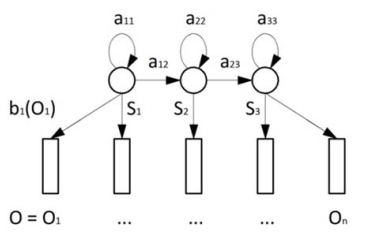
\includegraphics [width=.5\linewidth] {hmm}
	\caption{Топологія прихованих Марковських моделей з трьома станами}
	\label{img:hmm}
\end{figure}

\subsubsection{Динамічне трансформування часу}

Відомо, що мовний сигнал швидко змінюється в часі. Різні вимови одного і того ж слова зазвичай мають різну тривалість, а вимови одного і того ж слова однаковою тривалості відрізняються в середині через різні частини слова, які вимовляються з різною швидкістю. Щоб отримати оцінку розбіжності між двома мовними сигналами, представленими як вектори, має бути виконано вирівнювання за часом, який можна реалізувати за допомогою динамічного трансформування часу \cite{Goldenstein_2013}.

Динамічне трансформування часу є методом еластичного порівняння вектора спостережень з шаблоном, що зберігається. Вектор спостережень і шаблон лежать на відповідних осях сітки. Для кожного осередку сітки вираховується різниця між відповідними фрагментами вектора спостережень і шаблону. Оптимальне вирівнювання між вектором спостережень і шаблоном показано маршрутом, що проходить по сітці.

Метод динамічного трансформування часу працює з фрагментами, тобто аналіз ознак складається з обробки вектора ознак в регулярних інтервалах. Так як вектор ознак може мати безліч фрагментів, потрібні засоби розрахунку локальної оцінки відстані. Оцінка відстані між двома векторами ознак розраховується за допомогою Евклідової відстані.

Хоча обчислення Евклідової відстані в обчислювальному відношенні не вигідно в порівнянні з будь-якою іншою операцією, воно дає найкращі результати для розпізнавання.

\subsection{Недоліки традиційних систем розпізнавання мови}
Сучасні системи розпізнавання мови в більшій своїй частині засновані на статистичних методах, використовують потужний апарат теорії ймовірностей та математичної статистики, що дає змогу суттєво підвищити якість розпізнавання. Основні методи розпізнавання мови --- це приховані Марківські моделі та штучні нейронні мережі \cite{Makovkin_2006, Gefke_2012}. Але у сучасних системах більш поширеними є моделі на нейронних мережах, оскільки вони мають більшу швидкодію та стійкість до шумів \cite{Hinton_2012}.

Звісно, на вхід до нейронної мережі не подають «сирий» звук — амплітуду коливань по часу, адже це не дуже інформативна форма представлення акустичного сигналу для аналізу. Більш інформативним є спектр сигналу, але на практиці найчастіше використовується мел-перетворення, в якому звуковий сигнал нарізається на фрейми розміром 20–40 мс, спектр кожного з яких масштабується через банк фільтрів та логарифмується для отримання даних, найбільш наближених до людського сприйняття \cite{Saini_2013}.

Існує досить багато таких систем і вони доволі якісно виконують свою задачу. Але в більшості своїй ці системи розраховані на роботу в приміщеннях без сильних шумів, залучення дикторів з чіткою вимовою та використання потужних компʼютерів або віддалених серверів, як, наприклад, Google Voice Search. Та й ці системи неідеальні, в них не вирішені проблеми фільтрації шумів та розпізнавання великих обʼємів даних, обмежені можливості налаштування під різні умови та різних дикторів \cite{Volkov_2014}. Так, наприклад, в системах мовного управління бортовим обладнанням літаків мінімальна можлива якість становить 95\%, а час розпізнавання не повинен перевищувати 0,2 с при темпі мовлення порядку 100 слів за хвилину \cite{Bondaros_2007}. Навіть у рамках однієї системи розпізнавання ці параметри можуть змінюватися в залежності від багатьох факторів, у тому числі таких, що визначаються умовами польоту, різними акустичними перешкодами, впливом пілотажних перевантажень тощо. \cite{Korsun_2013}.

Дослідження по розпізнаванню мовлення показують необхідність великих контекстно-залежних словників а також великих корпусів для навчання системи \cite{Pylypenko_2008,Pylypenko_2009,Pylypenko_2010,Lydovyk_2011,Vasilyeva_2012,Womack_1999,Zirneeva_2008,Gladunov_2005}, однак акустичну модель навчену на великому корпусі можна використовувати для розпізнавання фонем у інших задачах, що не потребує словника \cite{Pylypenko_2008,Robeyko_2012,Abdel_2012,Zhang_2017,Sharma_2018,Yermolenko_2008}. 

Фактично, ті досягнення, які сьогодні здобуті в традиційних системах розпізнавання мови, вже можуть бути використані для забезпечення голосової взаємодії в управлінні дистрибуцією. Проте вони не в змозі повністю забезпечити автоматизацію голосової взаємодії в задачах управління дистрибуцією, оскільки немає можливості а ні встановити у кабіні водія потужне обладнання, а ні забезпечити стабільний та швидкісний доступ до інтернету. Крім того, кабіна водія — це неконтрольоване акустичне середовище з високим рівнем шуму. Проблема багатодикторності також актуальна для дистрибуції, адже у таких компаніях зазвичай працює від декількох десятків до кількох сотень і навіть тисяч водіїв, в яких можуть бути дефекти вимови, різноманітні акценти та інші індивідуальні особливості мовлення.

\subsection{Класифікація та виділення керуючої інформації з мовного сигналу}

%\paragraph{Speech classification}

У класифікації звуку можна виділити наступні основні категорії: класифікація емоційного забарвлення \cite{Ververidis_2004,Ververidis_2004_2,Ververidis_2006,Kaya_2017,Deb_2016,Bhaskar_2015,Devillers_2015,Weisskirchen_2017,Sharma_2018,Ozseven_2018}, визначення диктора \cite{Rabotyagov_2006} чи його особливостей (вік, стать) \cite{Kaya_2017}, виділення проміжків мовлення \cite{Hussain_2018,Khonglah_2016,Benatan_2015,Priya_2012} або інших класів звукового змісту (музика, фонових шумів, тощо) \cite{Hussain_2018,Boddapati_2017} у аудіозаписах, класифікація мовленнєвих актів за метою вислову \cite{Ko_2015,Choi_1999,Grosz_1995,En_2005,Kang_2013,Kim_2012,Lee_2002,Sridhar_2008,Webb_2005,Kang_2010,Hellbernd_2016,Su_2017}.

В деяких роботах аналіз може відбуватись за попередьньо отриманим текстом \cite{Ko_2015,Choi_1999,Grosz_1995,En_2005,Kang_2013,Kim_2012,Lee_2002,Webb_2005,Kang_2010}, в деяких виключно за звуковими характеристиками \cite{Ververidis_2004,Ververidis_2004_2,Ververidis_2006,Kaya_2017,Deb_2016,Devillers_2015,Weisskirchen_2017,Sharma_2018,Hussain_2018,Khonglah_2016,Benatan_2015,Priya_2012,Boddapati_2017,Hellbernd_2016}, а в деяких звук і текст використовуються разом \cite{Bhaskar_2015,Sridhar_2008,Chowdhury_2018}.

Важливе значення виділення мовлення з фонового шуму проявляється у задачі підсилення голосу для людей з погіршеним слухом. Зокрема це може бути реалізовано у додатку на смартфоні \cite{Vashkevich_2018}.

%\paragraph{Control instruction}

Більшість систем розпізнавання та розуміння управляючих команд зосереджені в сфері робототехніки. У переважній більшості підходів, розпізнавання керуючих команд відбувається за текстовим їх представленням, наприклад після автоматичного розпізнавання голосу. Деякі підходи зосереджені на спробах побудувати достатньо складну але чітку грамматику команд \cite{Misra_2016,Fasola_2013,Eppe_2016}, деякі гнучко класифікують заздалегідь заданий перелік команд \cite{Yongda_2018}, а найпростіші просто шукають задні ключові слова в тексті \cite{Shwe_2003,Shulika_2018}. Існують роботи в яких відбувається класифікація голосових команд без переводу в текст, але перелік команд лише обмежується декількома пунктами \cite{Shulika_2018,Gryshchuk_2006}.

%\paragraph{Text processing}

Як можна бачити з прикладів задач класифікації мовленнєвих актів та розпізнавання керуючих команд, аналіз змісту сказаного голосом, в переважній більшості випадків частково чи повністю відбувається через аналіз вже розпізнаного тексту сказаного, а значить переходить із задачі аналізу голосу, в сферу обробки та розуміння природної мови. Існує велике різноманіття методів обробки та класифікації природно-мовних текстів \cite{Mironczuk_2018,Altinel_2018,Hartmann_2018,Kim_2014,Britz_2015_2,Britz_2015,Marchenko_2005}.

%\paragraph{Phoneme usage} 

Використання фонемного тексту замість лексичного для роботи зі звуком було добре досліджено у задачі пошуку по звуковим файлам \cite{Ng_C_2000,Ng_K_2000,Witbrock_1997}. Результати показали що попри незначне зменшення якості пошуку, воно дає переваги в вирішені проблеми слів поза словником та може мати переваги в використанні на мобільних пристроях. Крім того були дослідження по автомоатичному визначенню та класифікації одиниць мовлення \cite{Sharma_2018}.

Підходи роботи з текстовими даними посимвольно \cite{Kim_2016,Zhang_2015_2,Zhang_2015,Santos_2014} можуть бути використані для пофонемної роботи з фонетичним текстом.

%\paragraph{CNN direct}

В деяких роботах для роботи зі звуком напряму чи зі спектрограмою звуку використовувалися згорткові нейронні мережі. А саме в задачах класифікації емоційного забарвлення \cite{Weisskirchen_2017}, класифікації звуків навколишнього середовища \cite{Boddapati_2017}, Визначення мети одночасного мовлення \cite{Chowdhury_2018}, розпізнавання послідовності фонем \cite{Abdel_2012,Zhang_2017}, та інших.

%\paragraph{Spoken dialogue systems}

Окремо розглядаються методи побудови голосових діалогових систем \cite{Iosif_2018}. Можна виділити голосові діалогові системи на основі правил \cite{Herbert_2018,Lopes_2015} та на основі сценаріїв \cite{Lopez_2016,Khouzaimi_2018}. Існують спеціальні методи опису та синхронізації багато модальних діалогових систем з використанням голосових даних \cite{Katsurada_2003,Karpov_2012}. 

\section{Новітні підходи до автоматизації голосової взаємодії} \label{sect1_5}

Японський дослідник з університету Осаки Ішігуро Хіроші з колегами вивчали різні аспекти комунікації та інформаційно-комунікаційних технологій, як, наприклад, використання комунікації з людиноподібними роботами в якості терапевтичної дії для людей похилого віку \cite{Nishio_2015}, аутистів \cite{Kumazaki_2016} чи просто замкнутих у собі людей, педагогічної дії щодо дітей та немовлят \cite{Park_2015} тощо. Зокрема він проводив дослідження голосової комунікації двох людей опосередковано через компʼютер \cite{Ishiguro_2016}. 

У цьому дослідженні пара спілкувалася на загальні теми, обираючи варіанти своєї репліки із заздалегідь написаного дерева варіантів, свого роду сценарію. Жодному з партнерів не потрібно було нічого промовляти вголос: людині надавався набір з варіантів реплік на вибір, потрібно було лише натиснути на ту з них, яку б вона хотіла  промовити, і ця репліка лунала з динаміків. У залежності від використаної репліки програма вибирала з дерева сценаріїв можливі варіанти відповідей і надавала їх на вибір співрозмовнику. Співрозмовник у свою чергу, чуючи репліку першої людини, обирав свою з поданих варіантів. Це дослідження було спрямоване на подолання соромʼязливості при спілкуванні з особами протилежної статі (що є особливо актуальним для Японії). Але такий підхід заздалегідь написаного дерева сценаріїв комунікації можна використовувати і в інших сферах.

У доповіді на світовому психологічному конгресі 2016 проф. Ішігуро демонстрував використання цього сценарного підходу для роботів на виставках та в музеях. Що б уникнути необхідності розпізнавання голосу в шумному середовищі, поряд з експонатом ставиться людиноподібний робот та монітор, на якому показані варіанти запитань. Натискаючи на різні репліки, відвідувач може спілкуватися з роботом по заздалегідь написаному дереву сценаріїв, розпитуючи його про експонат, а робот буде відповідати голосом.

На жаль для управління дистрибуцією постає зворотне завдання — водій має повідомити певну інформацію в систему і при цьому не повинен відволікатися на натискання кнопок на екрані. Тому пряме використання такої технології неможливе. Але застосування підходу описання всіх можливих сценаріїв комунікації в залежності від контексту дозволить знизити кількість інформації, яку треба розпізнати, а отже і підвищити якість.

Наразі існує новий підхід до голосового управління, заснований на теорії несилової взаємодії \cite{Teslia_2010} — рефлекторна система голосового управління \cite{Egorchenkov_2016}. Ідея, покладена в основу цього підходу, полягає в тому, щоб замість переведення голосової інформації в текстову репрезентацію, аналізувати безпосередньо інформаційну складову сказаного, визначаючи, яку з відомих реакцій потрібно виконати. «Традиційні системи розпізнавання мови засновані на принципі: „усна мова“ → „репрезентація мови набором лінгвістичних конструкцій“ → „розуміння мови“. На основі теорії несиловой взаємодій може бути запропонована інша модель розпізнавання природної мови: „усна мова“ → „розрахунок несилової (інформаційної) взаємодії на реакції“ → „реакція (розуміння чи поведінка)“» \cite{Teslia_2014}.

Така модель розпізнавання називається рефлекторною, оскільки побудована за аналогією зі структурою умовного рефлексу, в якому виділяються афектори, центральний компонент та ефектори. Така модель може бути добре поєднана з ідеєю використання дерева сценаріїв, оскільки сценарії також складаються із реакцій, і одиницею моделювання стає не лінгвістична особливість мовлення, а реакція (або команда), яка може бути врахована автоматизованою системою розрахунку маршрутів. Тобто, суть цього підходу полягає в тому, щоб перейти до іншої одиниці розпізнавання мови. У психології дискурсивного мислення і рефлексивній психології також накопичено досвід аналізу мови, через виокремлення інших одиниць — функціональних висловлювань \cite{Naydonov_2008}.

Оскільки в такій системі не потрібні словники, складні інтелектуальні моделі аналізу тексту та граматики, вони мають низку переваг порівняно з традиційними системами: багатодикторність, варіабельність природної мови, можливість обробки команд офлайн прямо на пристрої, робота в умовах шумів (неконтрольованого акустично середовища), простота алгоритмів та менша складність і ціна реалізації \cite{Teslia_2013}.

У загальному випадку система рефлекторного голосового управління складається з трьох компонентів:

1. \textit{Фонемний стенограф}

Відповідає за перетворення відцифрованого вхідного звукового сигналу, що поміщає усну мову в набір фонем або слів.

2. \textit{Ядро системи}

Здійснює моделювання системи голосового управління. Містить програмну реалізацію всіх моделей, методів та алгоритмів системи, набір команд, протокол роботи, налаштування тощо.

3. \textit{База даних розпізнавання мови з можливістю навчання}

Забезпечує зберігання інформаційної бази розпізнавання мови та виділення керуючого впливу. У базі даних зберігається статистика вхідних впливів та відповідних їм вихідних реакцій системи.

Варто зазначити, що модуль фонемного стенографа може бути забезпечений різними програмними засобами, що робить систему гнучкішою та більш адаптивною до умов середовища. Єгорченков \cite{Egorchenkov_2016} наводить перелік можливих модулів фонемного стенографа. Провівши порівняльне зіставлення стенографів з цього переліку, можна стверджувати, що найбільш прийнятним для задач дистрибуції є фонетичний стенограф на основі Julius speech recognition tool \cite{Pylypenko_2009}, оскільки він у своїй роботі не потребує ні доступу до інтернету, ні великих словникових баз, а дає на виході «сирі» фонеми (наприклад, «п ъ й! А м а» для слова «Прямо»), які можуть навіть краще сприйматися рефлекторною системою для подальшого визначення інформаційного компоненту, ніж розпізнані слова, через вищу (в останньому випадку) ймовірність помилки.

\section{Постановка задачі дослідження} \label{sect1_6}

\textbf{Наукова задача} дисертаційної роботи полягатиме в розробці моделей і методів формалізації голосової інформації в системах диспетчерського контролю за рухом автотранспорту.

У процесі вирішення наукової задачі висунута наступна \textbf{гіпотеза}, що поєднання двох найбільш перспективних напрямків, дає змогу запропонувати нове принципове рішення і побудувати рефлекторну модель голосової взаємодії в задачах управління дистрибуцією.


\textbf{Основна ідея} даної наукової роботи полягає в тому, що розроблення моделі голосової взаємодії без блоку переведення звуку голосу в текст може принципово покращити автоматизацію голосової взаємодії в системах контролю дистрибуції.

\textbf{Дослідження}, результати яких викладені в подальших розділах цієї роботи, спрямовані:

\begin{itemize}
	\item на визначення методики досліджень і побудови науково-методологічних основ автоматизації голосової взаємодії (розділ 2);
	\item на розробку методів формалізації голосової інформації в системах диспетчерського контролю за рухом автотранспорту (розділ 3);
	\item на створення засобів формалізації голосової інформації в системах диспетчерського контролю за рухом автотранспорту(розділ 4).
\end{itemize}

\section*{Висновки до розділу 1}
\addcontentsline{toc}{section}{Висновки до розділу 1}

1. Розглянувши проблему формалізації голосової інформації в системах диспетчерського контролю за рухом автотранспорту встановлено, що інформаційні технології в управлінні дистрибуцією є достатньо розробленими для забезпечення етапів отримання продукції та її збереження, але недостатньо --- для етапу доставки продукції до кінцевих клієнтів, особливо щодо проблеми «останньої милі». Значну роль в управлінні дистрибуцією відіграють процеси голосової взаємодії, автоматизація яких здатна підвищити ефективність системи дистрибуції.

2. На сучасному етапі автоматизації голосового управління в організаційно-технічних системах існує проблема своєчасного коригування в необхідних випадках планових маршрутів руху автотранспорту, що інколи призводить до достатньо великих витрат часу на комунікацію, і відповідно є найбільш обґрунтованим напрямом автоматизації голосової взаємодії.

3. Автоматизація голосової взаємодії для своєчасного коригування планових маршрутів руху автотранспорту повинна доповнити наявні засоби автоматизації управління в системах дистрибуції, такі як відстеження руху автомобілів у режимі реального часу за допомогою GPS треку. Існуючі в дистрибуції системи автоматизації голосової взаємодії для управління зберіганням є занадто спрощеними для використання в задачах доставки.

4. Проведений аналіз сучасних інформаційних систем формалізації голосової інформації показав, що традиційно вони включають три етапи: попередня обробка з виділенням ознак, перетворення голосової інформації в текстову та виділення змісту з текстової інформації. Такий підхід не в змозі повністю забезпечити автоматизацію голосової взаємодії в задачах управління дистрибуцією, оскільки переведення голосової інформації в лексичний текст потребує встановлення у кабіні водія потужного обладнання або забезпечення стабільного та швидкісного доступу до Інтернету. Висунуто ідею, що розроблення моделі голосової взаємодії без блоку переведення звуку голосу в текст може принципово покращити автоматизацію голосової взаємодії в системах контролю дистрибуції.

5. Встановлено пріоритетність підходу до голосового управління, заснованого на теорії несилової взаємодії з рефлекторною системою голосового управління. Підхід включає безпосередній аналіз інформаційної складової, вимовленої субʼєктом, з визначенням керуючого впливу з поміж відомих реакцій в певному предметному полі.

6. В результаті проведеного аналізу сформована основна ідея, гіпотеза, мета та спрямування дослідження, поставлено задачі досліджень дисертаційної роботи. Визначена необхідність в розробці моделей і методів, що дадуть змогу формалізувати голосову інформацію в системах диспетчерського контролю за рухом автотранспорту, тим самим забезпечити підвищення ефективності управління системою дистрибуції.

